% Chapter Template

\chapter{Analysis and Findings} % Main chapter title

\label{Chapter3} % Change X to a consecutive number; for referencing this chapter elsewhere, use \ref{ChapterX}

%----------------------------------------------------------------------------------------
%	SECTION 1
%----------------------------------------------------------------------------------------

\section{Logistic Regression}

I first compute the average SF ratio per ICU stay.  Next, I fit the following logistic regression :
\setlength\abovedisplayskip{4pt}
\setlength\belowdisplayskip{4pt}
\begin{equation*}
\ln \left(\frac{M}{1-M}\right)=\beta_{0}+\beta_{1} (\text{Average SF Ratio})+\beta_{2} (\text{Gender}) + \beta_{3} (\text{Age}) + \beta_{4} (\text{BMI}) + \beta_{5} (\text{Sofa Total Score}) 
\end{equation*}
where $M$ is Hospital Mortality, BMI is the Body Mass Index of the patient and Sofa Total Score is a  .  The results are as follows:

\begin{table}[H] 
\centering
\begin{tabular}{|l|c|c|c|c|}
\hline
\textbf{Feature} & \multicolumn{1}{l|}{\textbf{Estimate}} & \multicolumn{1}{l|}{\textbf{Std. Error}} & \multicolumn{1}{l|}{\textbf{z-value}} & \multicolumn{1}{l|}{\textbf{p-value}} \\ \hline
Intercept & -0.3427213 & 0.2362569 & -1.451 & 0.147 \\ \hline
Average SF Ratio & -0.0097838 & 0.0008024 & -12.193 & \textless 2e-16 \\ \hline
Gender (M) & -0.3579267 & 0.0585947 & -6.109 & 1.01e-09 \\ \hline
Age & 0.0045151 & 0.0005280 & 8.551 & \textless 2e-16 \\ \hline
BMI & -0.0316707 & 0.0044837 & -7.063 & 1.62e-12 \\ \hline
Sofa Total Score & 0.1964941 & 0.0083214 & 23.613 & \textless 2e-16 \\ \hline
\end{tabular}
\caption{Results of Logistic Regression}
\label{tab:logisitic}
\end{table}

Hence, the Average SF ratio is significantly correlated with Hospital Mortality and a unit increase in SF ratio decreases odds of
hospital mortality by 1.19\%.  

%----------------------------------------------------------------------------------------
%	SECTION 2
%----------------------------------------------------------------------------------------

\section{Generalized Additive Model}

A logistic regression assumes a linear relationship between mortality and the different features which may not necessarily be true. To explore a potential non-linear relationship I use a generalised additive model. A generalized additive model is an extension of a generalized linear model with a linear predictor involving a sum of smooth functions of covariates \citep{hastie2017generalized}. The general model can be expressed as follows \citep{wood2017generalized}: 
\setlength\abovedisplayskip{4pt}
\setlength\belowdisplayskip{4pt}
\begin{equation*}
g\left(\mu_{i}\right)=\mathbf{A}_{i} \boldsymbol{\theta}+f_{1}\left(x_{1 i}\right)+f_{2}\left(x_{2 i}\right)+f_{3}\left(x_{3 i}, x_{4 i}\right)+\ldots
\end{equation*}

where  \(Y_{i} \sim \operatorname{EF}\left(\mu_{i}, \phi\right), Y_{i}\) is the response variable, \(\mu_{i} \equiv \mathbb{E}\left(Y_{i}\right)\) and \(\mathrm{EF}\left(\mu_{i}, \phi\right)\) denotes
an exponential distribution with mean \(\mu_{i}\) and parameter, \(\phi\). Also, \(f_{j}\) are smooth functions of the covariates, \(x_{k}\) \citep{wood2017generalized}. 

Now fitting a GAM model to our data with Hospital Mortality as response variable and a smoothening function applied to predictors Average SF Ratio, Age and Length of ICU Stay and Gender taken as a linear predictor. We obtain the following results: 


\begin{table}[H]
\begin{tabular}{|l|l|l|l|l|}
\hline
\textbf{Feature}         & \textbf{edf} & \textbf{Ref.df} & \textbf{Chi.sq} & \textbf{p-value} \\ \hline
Average SF Ratio          & 6.968        & 8.078           & 957             & \textless{}2e-16 \\ \hline
Age                   & 5.582        & 6.665           & 411.2           & \textless{}2e-16 \\ \hline
Length of ICU Stay& 5.262        & 6.268           & 306.8           & \textless{}2e-16 \\ \hline
\end{tabular}
\caption{Results of GAM}
\label{tab:GAM}
\end{table}

The result of the model in table \ref{tab:GAM} shows that there is a statistically significant correlation between Hospital Mortality and Average SF Ratio. I visualize this relationship below in fig \ref{fig:GAM}. The visualizations for all the predictors can be found in Appendix \ref{AppendixA}. 

\begin{figure}[H]
  \centering
    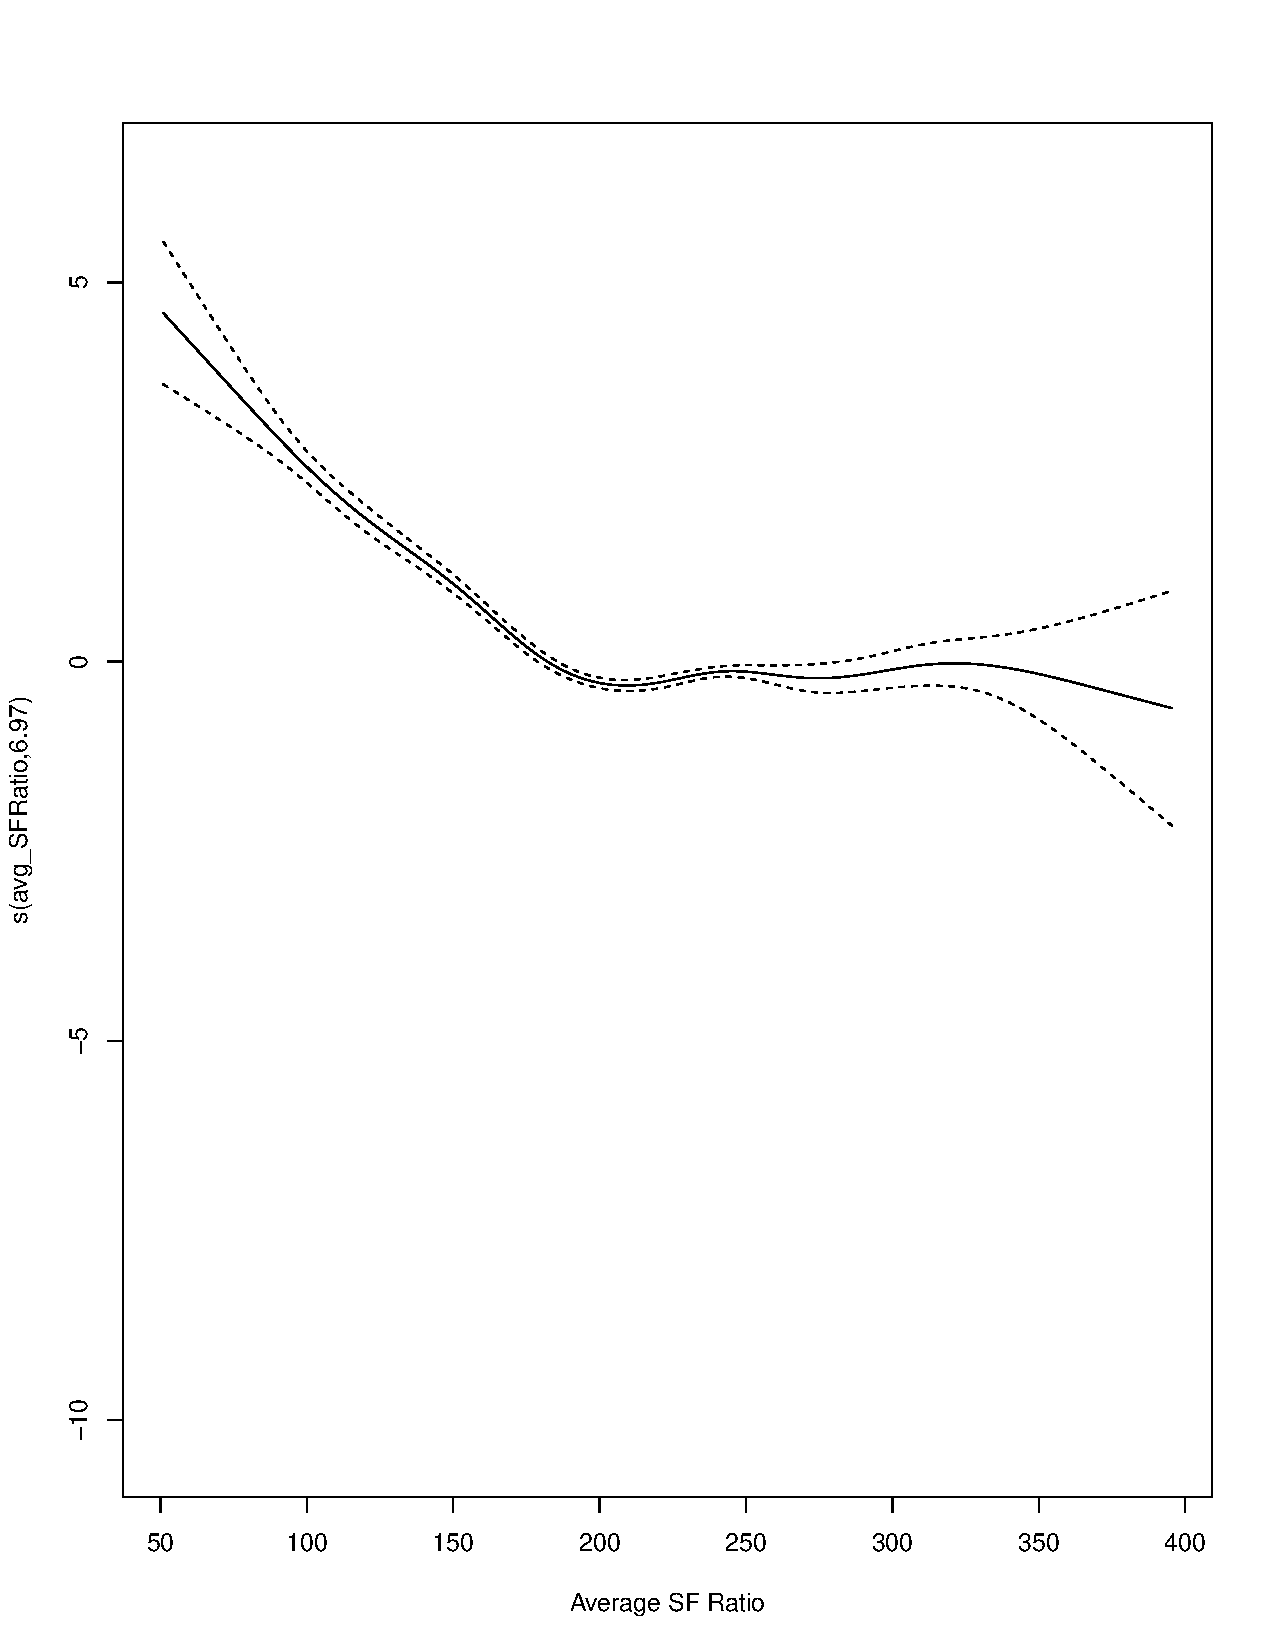
\includegraphics[width=0.9\textwidth]{figures/GAM-AVGSF.pdf}
  \caption{Results of GAM model for relationship between Average SF Ratio and log odds of Hospital Mortality}
  \label{fig:GAM}
\end{figure}

From fig \ref{fig:GAM} we see that a increase in Average SF Ratio from around 100 to around 200 causes a reduction in the log odds of Hospital Mortality with minimal standard error.  

